%!TEX root = ../main.tex

\chapter{Future updates, trivia and conclusions}
\label{chp:conclusions}

\section{Needed work}
\noindent
The project is far from finished and requires additional work. The following paragraphs will outline the major updates needed.

\paragraph{Security}
There are significant security vulnerabilities, particularly in the backend, which currently lacks any form of protection. It needs a system for user authentication and token creation for both the \ac{VR} app and the web app.
Additionally, the \ac{VR} app will require a user-friendly authentication interface that enables end users to authenticate themselves without difficulty.

\paragraph{Ready for the store}
The app is far from being ready for the Meta Quest store. It needs to implement internet multiplayer and achieve a more stable frame rate when loading 3D models.
Additionally, it may require a new algorithm for creating \ac{LOD}s in real time.

\paragraph{Future features}
The app needs to be updated for new version of Meta OS, and the app could benefit from some other functionality like:

\begin{itemize}
  \item Online multiplayer
  \item	Slicing 3D models
  \item	3D models caching 
  \item	New environments
\end{itemize}

\section{Science4All}
\noindent
Science4All is a science outreach and inclusion project in Padua, aimed at making complex scientific topics accessible to a broad audience,
from young people to adults without a scientific background, with particular attention to people with disabilities or from disadvantaged backgrounds.\\
For the occasion, the \ac{VR} app was presented in the 3D printing section focused on medical applications. In a specially designed environment Fig.[\ref{fig:science4all}], we allowed children to try the \ac{HMD}, for many, it was their first time experiencing VR. They had the opportunity to view a heart model, exploring both the exterior and interior in detail.
Both children and parents were captivated by the app capabilities and the medical use case for which it was developed.

\begin{figure}[ht]
  \centering
  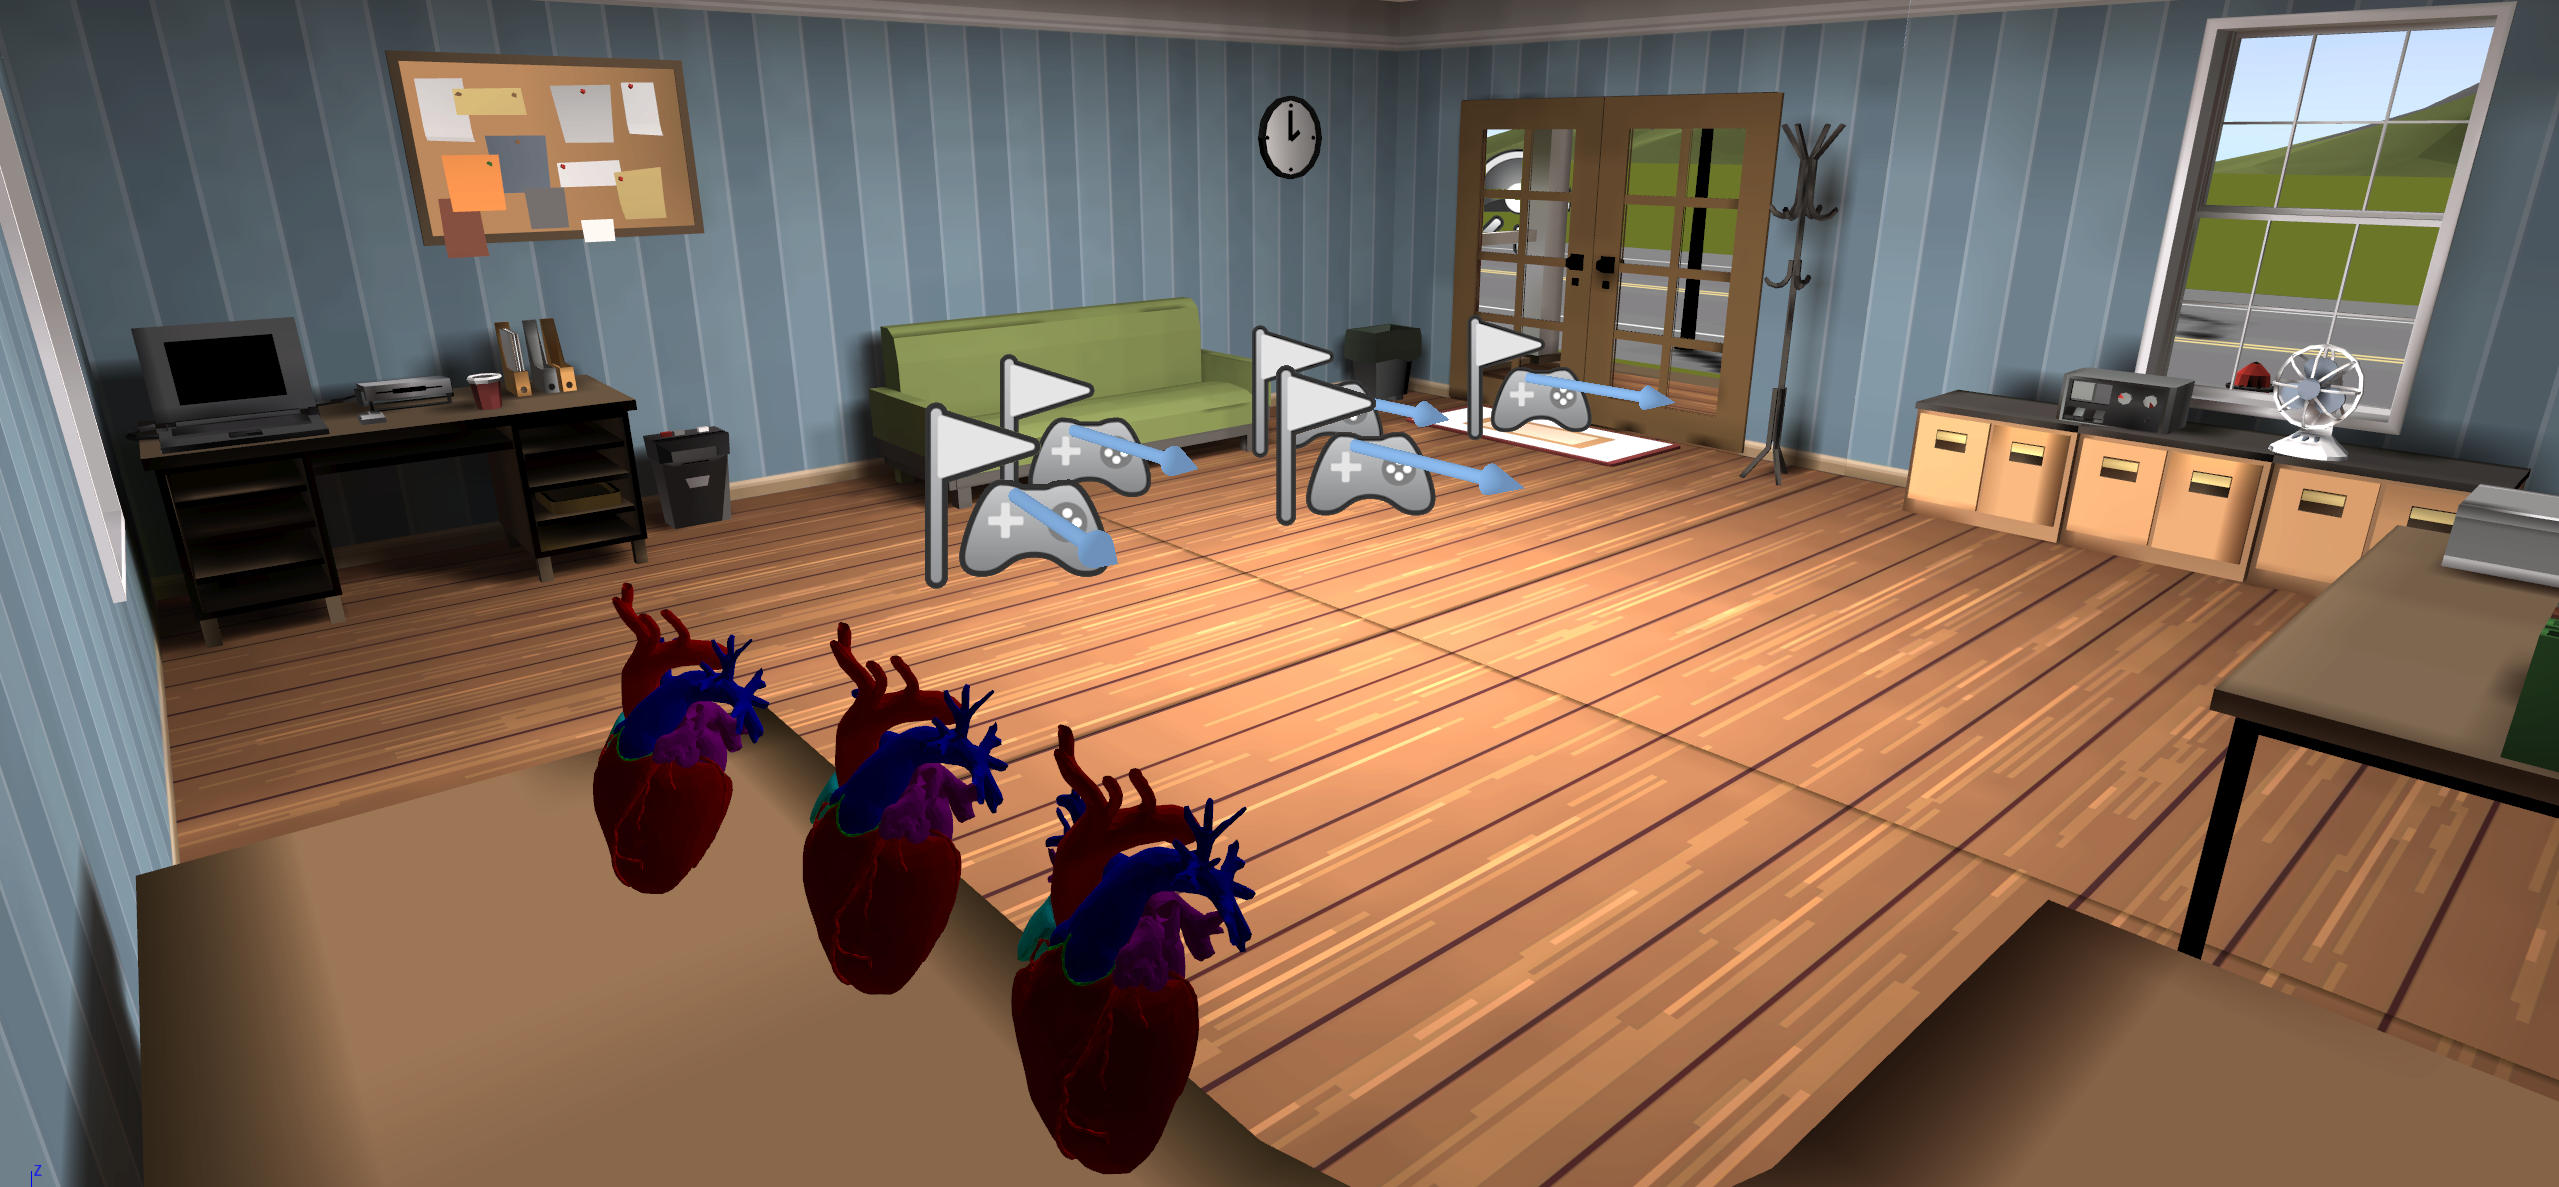
\includegraphics[width=\textwidth]{vrScreenshot/science4all.png}
  \caption{Science4All environment}
  \label{fig:science4all}
\end{figure}